\documentclass[aspectratio=169,10pt]{beamer}

\usepackage[T1]{fontenc}
\usepackage[utf8]{inputenc}
\usefonttheme{serif}
\usepackage{mathpazo}
\usepackage[american]{babel}
\usepackage{csquotes}
\usepackage[backend=biber,style=apa]{biblatex}
\addbibresource{references.bib}
\graphicspath{{assets/}}

\usepackage{amssymb}
\usepackage{booktabs,array,colortbl,microtype}
\usepackage{tikz}
\usetikzlibrary{arrows.meta,positioning,calc,shapes.geometric,fit,backgrounds}

% --- Settings & Definitions (adapted from the supplied role-model template) ---
\newcommand{\defencedate}{19 November 2026\par}
\newcommand{\imgdir}{assets/}
\newcommand{\logofile}{SU_Logo.png}

% Palette sampled from the Strathmore website and crest (supplied template).
\definecolor{StrathNavy}{HTML}{1C1B3B}
\definecolor{StrathBlue}{HTML}{3F73B5}
\definecolor{StrathGold}{HTML}{F4B218}
\definecolor{StrathRed}{HTML}{C50227}
\definecolor{StrathLight}{HTML}{EEF2F8}
\definecolor{StrathInk}{HTML}{1F2A44}

\newcommand{\StrathLogo}[1]{%
  \IfFileExists{\imgdir\logofile}{\includegraphics[height=#1]{\imgdir\logofile}}%
  {{\scriptsize\bfseries\color{StrathNavy}Strathmore University}}}

% --- Theme: preserve the supplied role-model structure and tweaks ---
\usetheme{default}
\setbeamertemplate{navigation symbols}{}
\setbeamersize{text margin left=1cm,text margin right=1cm}
\setbeamercolor{normal text}{fg=StrathInk}
\setbeamercolor{structure}{fg=StrathBlue}
\setbeamercolor{frametitle}{fg=StrathNavy}
\setbeamercolor{footline}{fg=white,bg=StrathNavy}
\setbeamercolor{block title}{fg=white,bg=StrathNavy}
\setbeamercolor{block body}{fg=StrathInk,bg=StrathLight}
\setbeamerfont{frametitle}{size=\large,series=\bfseries}
\setbeamerfont{block title}{size=\small,series=\bfseries}
\setbeamerfont{block body}{size=\small}
\setbeamerfont{footnote}{size=\tiny}
\setbeamertemplate{itemize item}{\color{StrathRed}\tiny$\blacksquare$}
\setbeamertemplate{itemize subitem}{\color{StrathBlue}\tiny$\blacktriangleright$}
\setlength{\leftmargini}{1.1em}
\setbeamertemplate{blocks}[rounded][shadow=false]
\setbeamertemplate{bibliography item}{}

\setbeamertemplate{frametitle}{%
  \vskip1.6mm
  {\leftskip=0cm \rightskip=1.7cm plus 1fil \parindent=0pt
   \usebeamerfont{frametitle}\usebeamercolor[fg]{frametitle}\insertframetitle\par}
  \vskip1.2mm
  {\color{StrathRed}\rule{2.6cm}{1.6pt}}\par
  \vskip0mm}

\setbeamertemplate{headline}{%
  \vbox to 0pt{\vskip1.5mm\hbox to \paperwidth{\hfill\StrathLogo{0.95cm}\hspace{0.45cm}}\vss}}

\newcommand{\trk}[2]{\ifnum0\insertsectionnumber=#1\relax
  \textcolor{StrathGold}{\bfseries #2}\else\textcolor{white!55!StrathBlue}{#2}\fi}

\setbeamertemplate{footline}{%
  \leavevmode\hbox{%
   \begin{beamercolorbox}[wd=.82\paperwidth,ht=2.5ex,dp=1.1ex,leftskip=1cm]{footline}
     \scriptsize\trk{1}{Context}\hspace{1.2em}\trk{2}{Intervention}\hspace{1.2em}%
     \trk{3}{Results}\hspace{1.2em}\trk{4}{Conclusion}
   \end{beamercolorbox}%
   \begin{beamercolorbox}[wd=.18\paperwidth,ht=2.5ex,dp=1.1ex,rightskip=1cm,right]{footline}
     \scriptsize\insertframenumber\,/\,\inserttotalframenumber
   \end{beamercolorbox}}\vskip0pt}

% Speaker notes: build two PDFs from this same source.
% Default (reading copy): slides followed by readable note pages.
% Define \PympressMode at compile time for notes on the right-hand screen.
\setbeamertemplate{note page}[plain]
\setbeamerfont{note page}{size=\small}

\def\PympressMode{} % Uncomment this line when ready for Pympress
\ifdefined\PympressMode
  \setbeameroption{show notes on second screen=right}
\else
  \setbeameroption{hide notes}
\fi

\hyphenpenalty=10000 \exhyphenpenalty=10000 \tolerance=2000 \emergencystretch=2em

% Helpers retained from the supplied template.
\newcommand{\stat}[3]{%
  \begin{tikzpicture}[baseline=(n.north)]
   \node[anchor=north west,rounded corners=3pt,fill=StrathLight,draw=StrathBlue!45,line width=.5pt,
         inner sep=4pt,text width=3.85cm,align=left,minimum height=1.30cm] (n)
     {{\large\bfseries\color{StrathBlue}#1}\\[-2pt]{\scriptsize #2 #3}};
  \end{tikzpicture}}
\newcommand{\pill}[1]{\tikz[baseline=(t.base)]\node[fill=StrathBlue,text=white,rounded corners=2pt,
  inner xsep=5pt,inner ysep=2pt,font=\scriptsize\bfseries](t){#1};}
\newcommand{\takeaway}[1]{\par\vfill{\centering\color{StrathBlue}\bfseries #1\par}\vspace{1mm}}
\newcommand{\smallcite}[1]{{\scriptsize\color{StrathInk!75}#1}}

\title{Gaia DR3 Stellar Clustering}
\subtitle{An End-to-End Machine Learning Pipeline}
\author{Wesley Mwangi Gathua}
\institute{Strathmore University}

\begin{document}

% =====================================================================
% COVER (not counted)
% =====================================================================
\begin{frame}[plain,noframenumbering]
\begin{tikzpicture}[remember picture,overlay]
 \fill[StrathNavy] (current page.south west) rectangle (current page.north east);
 \fill[StrathRed] (current page.south west) rectangle ([xshift=0.35cm]current page.north west);
 % The supplied photograph is illustrative only; it is NOT a Gaia DR3 model result.
 % TODO: add the photograph's source/credit if required by its original licence.
 \node[anchor=south east,inner sep=0pt] at ([xshift=-0.8cm,yshift=0.9cm]current page.south east)
   {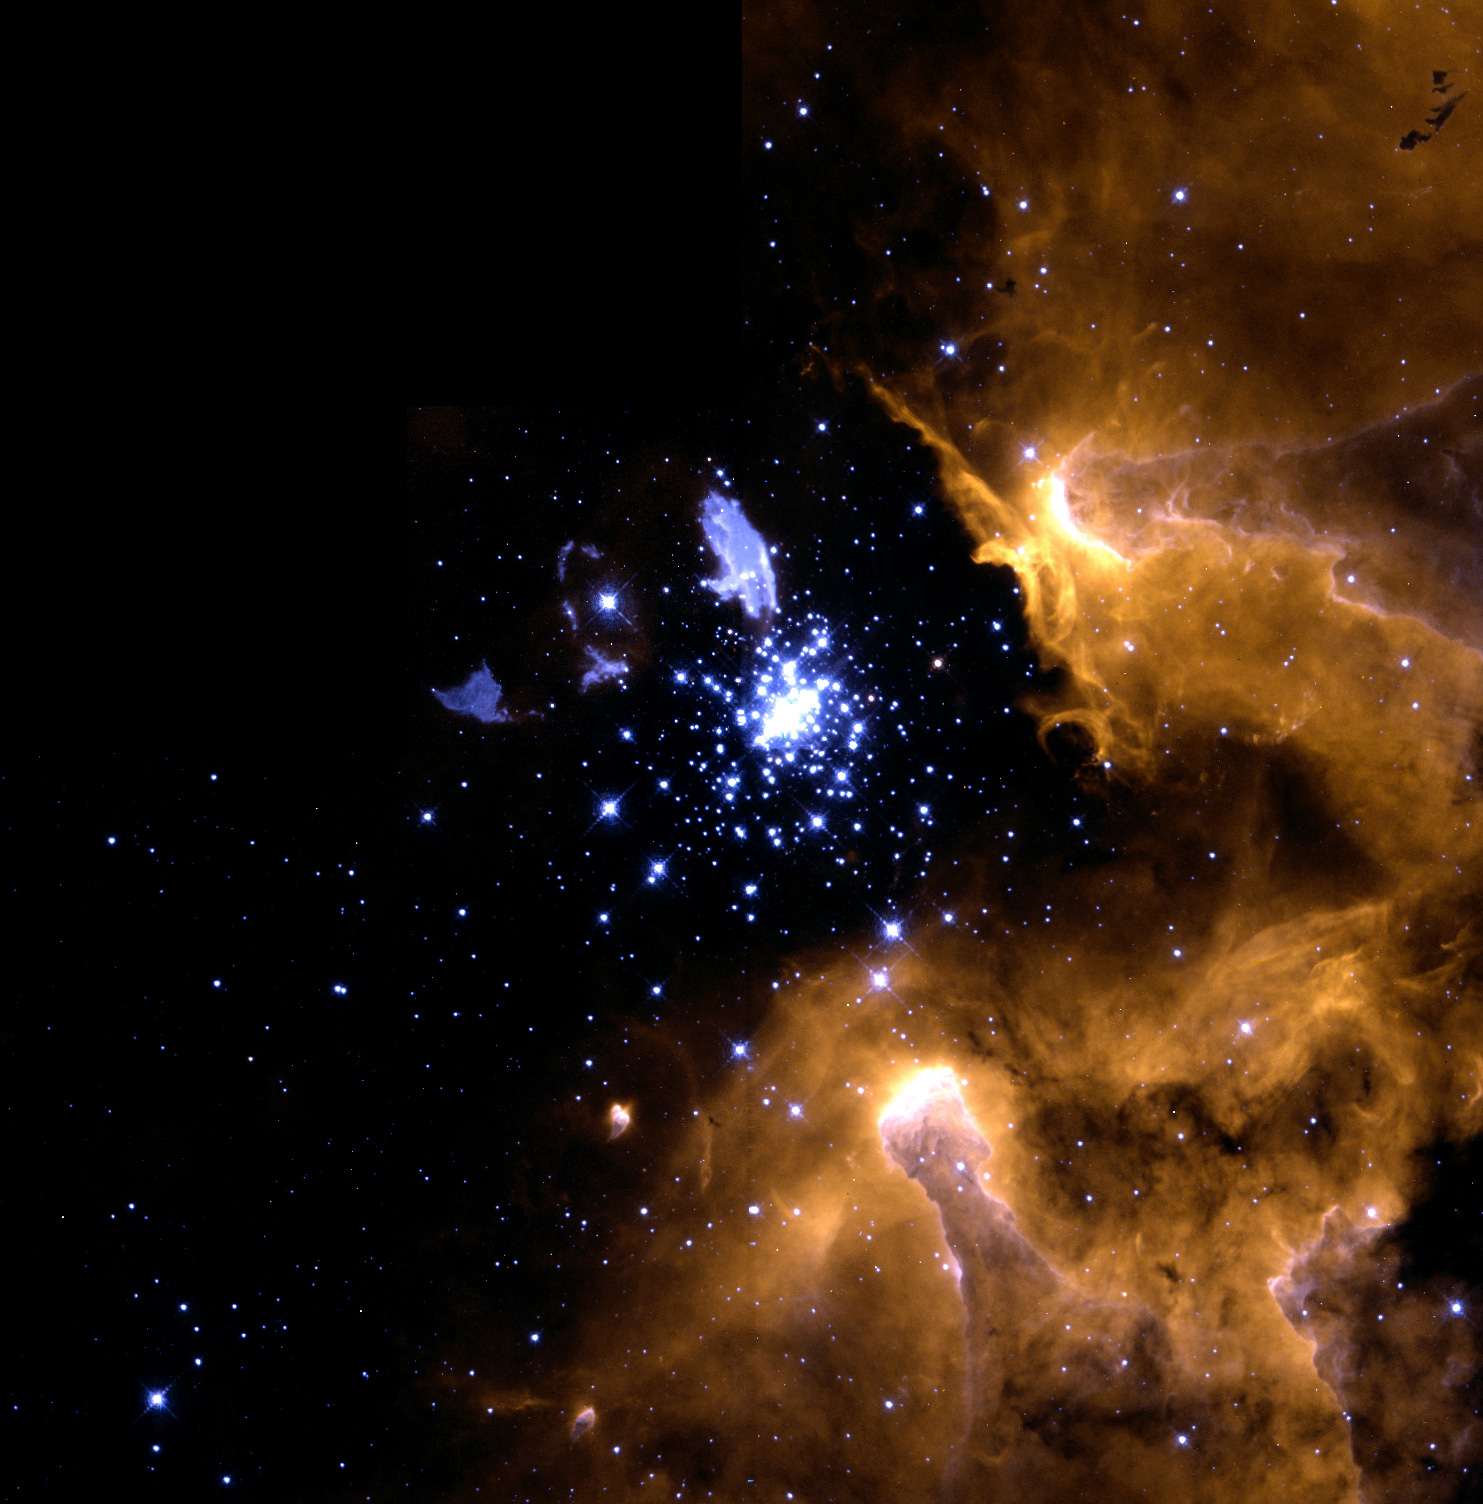
\includegraphics[width=5.05cm,height=5.45cm,keepaspectratio]{opo9920a.jpg}};
 \node[anchor=north east,text=white,align=right,text width=5.0cm,font=\tiny]
   at ([shift={(-0.8cm,-6.55cm)}]current page.north east)
   {.};
 \node[fill=white,rounded corners=5pt,inner sep=5pt,anchor=north east]
   at ([shift={(-0.8cm,-0.75cm)}]current page.north east){\StrathLogo{1.75cm}};
 \node[anchor=north west,text width=7.45cm,text=white,align=left]
   at ([shift={(1.1cm,-0.65cm)}]current page.north west){%
   {\small\bfseries STRATHMORE UNIVERSITY}\\[-1pt]
   {\scriptsize MSc DATA SCIENCE AND ANALYTICS  |  APPLIED MACHINE LEARNING}\\[4mm]
   {\LARGE\bfseries GAIA DR3\\[-1pt] STELLAR CLUSTERING}\\[1mm]
   {\color{StrathRed}\rule{2.8cm}{2.2pt}}\\[2mm]
   {\large An End-to-End Machine Learning Pipeline}\\[2mm]
   {\normalsize Exploratory analysis of 249,295 Gaia DR3 sources}\\[4mm]
   {\normalsize Wesley Mwangi Gathua  |  Reg. No. 223347}\\[1mm]
   {\scriptsize Lecturers: Prof. Javier Serrano \& Emmanuel Lee Bundi}\\[1mm]
   {\small 19 November 2026}};
\end{tikzpicture}
\note{\textbf{[About 5 seconds]} Good morning. This project uses unsupervised machine learning to explore a selected Gaia DR3 sample and delivers a reproducible pipeline with a tested local API. I will focus on why the task matters, how the two clustering views differ, and what the results do - and do not - establish.}
\end{frame}

% =====================================================================
\section{Context}
% =====================================================================

% ---------------------------------------------------------------------
\begin{frame}{A 249,295-source Gaia sample is rich in measurements but lacks complete motion data}
\noindent\stat{249,295}{sources in the selected Gaia DR3 sky window}{\parencite{gaia2016,gaia2023}}\hfill
\stat{83.13\%}{with radial velocity missing in the raw sample}{\parencite{gaia2023}}\hfill
\stat{6}{engineered features used for clustering}\\
\vspace{1mm}
\begin{columns}[T]
 \begin{column}{0.53\textwidth}
  \begin{itemize}\setlength{\itemsep}{5pt}
   \item The sample covers right ascension 50\textdegree--70\textdegree and declination $-5$\textdegree--$+5$\textdegree.
   \item No labelled target or external catalogue cross-match was used to establish cluster identities.
   \item Inputs combine position, sky-plane motion and photometry: $x,y,z$, tangential velocity, absolute $G$ magnitude and $BP-RP$ colour.
  \end{itemize}
 \end{column}
 \begin{column}{0.43\textwidth}
  \begin{block}{Astronomy terms, in plain language}
   \footnotesize
   \textbf{Parallax:} apparent position shift as the observing viewpoint changes; used here to estimate distance.\\[2pt]
   \textbf{Proper motion:} angular movement across the sky; with distance it gives tangential velocity.\\[2pt]
   \textbf{Radial velocity:} motion towards or away from us; it was not used because it is missing for most of this sample.
  \end{block}
 \end{column}
\end{columns}
\note{\textbf{[About 30 seconds]} The project does not analyse all of Gaia DR3. It uses a selected sky window with 249,295 sources. Gaia provides position, parallax, proper motion and photometry, but radial velocity is missing for about 83 percent of this sample. I therefore use tangential velocity, which captures motion across the sky, rather than claiming a full three-dimensional velocity. The six features combine ICRS-based position, tangential velocity and photometry. Importantly, there are no trusted labels or external catalogue matches in this experiment, so the task is exploratory clustering rather than classification against known astrophysical truth. Parallax is the apparent shift used to estimate distance; proper motion is the apparent angular movement across the sky.}
\end{frame}

% =====================================================================
\section{Intervention}
% =====================================================================

% ---------------------------------------------------------------------
\begin{frame}{K-Means partitions every source; UMAP--HDBSCAN can leave diffuse sources unassigned}
\begin{columns}[T]
 \begin{column}{0.47\textwidth}
  \begin{block}{K-Means: a complete baseline}
   \begin{itemize}\setlength{\itemsep}{4pt}
    \item Requires a chosen number of clusters; this project uses $k=4$.
    \item Assigns every source to one centroid-based group.
    \item Useful as a simple partition, but it cannot label diffuse points as noise. \smallcite{\parencite{macqueen1967}}
   \end{itemize}
  \end{block}
 \end{column}
 \begin{column}{0.49\textwidth}
  \begin{block}{UMAP--HDBSCAN: a density view}
   \begin{itemize}\setlength{\itemsep}{4pt}
    \item Standardise six features, then map them to a 2D neighbourhood representation with UMAP.
    \item HDBSCAN extracts dense groups without fixing $k$ in advance.
    \item Points outside selected density criteria receive label $-1$ (noise/unassigned). \smallcite{\parencite{mcinnes2018,campello2013}}
   \end{itemize}
  \end{block}
 \end{column}
\end{columns}
\vspace{1mm}
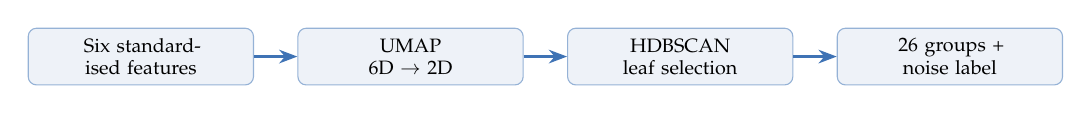
\begin{tikzpicture}[node distance=0.45cm and 0.55cm,
  bx/.style={rounded corners=3pt,draw=StrathBlue!55,fill=StrathLight,minimum height=0.72cm,text width=2.65cm,align=center,font=\scriptsize,inner sep=3pt},
  ar/.style={-{Stealth},thick,StrathBlue}]
  \node[bx] (x) {Six standardised features};
  \node[bx,right=of x] (u) {UMAP\\6D $\rightarrow$ 2D};
  \node[bx,right=of u] (h) {HDBSCAN\\leaf selection};
  \node[bx,right=of h] (o) {26 groups +\\noise label};
  \draw[ar] (x)--(u); \draw[ar] (u)--(h); \draw[ar] (h)--(o);
\end{tikzpicture}
\takeaway{These are complementary views of the same sample - not a contest using directly comparable scores.}
\note{\textbf{[About 35 seconds]} The critical modelling choice is that K-Means and HDBSCAN answer different questions. K-Means requires us to choose four clusters and assigns every source to one of them. That gives a useful coarse baseline, but a centroid method cannot leave diffuse observations unassigned. The second path standardises all six features, uses UMAP to create a two-dimensional representation, and then applies HDBSCAN. UMAP is designed to preserve important local neighbourhood relationships, but it can change the geometry and density of the data. HDBSCAN builds density-based groups and can label points that do not meet its selected density criteria as minus one. That label means unassigned under this model; it is not a physical class.}
\end{frame}

% ---------------------------------------------------------------------
\begin{frame}{A scripted pipeline turns the analysis into a reproducible, containerised service}
\begin{center}
 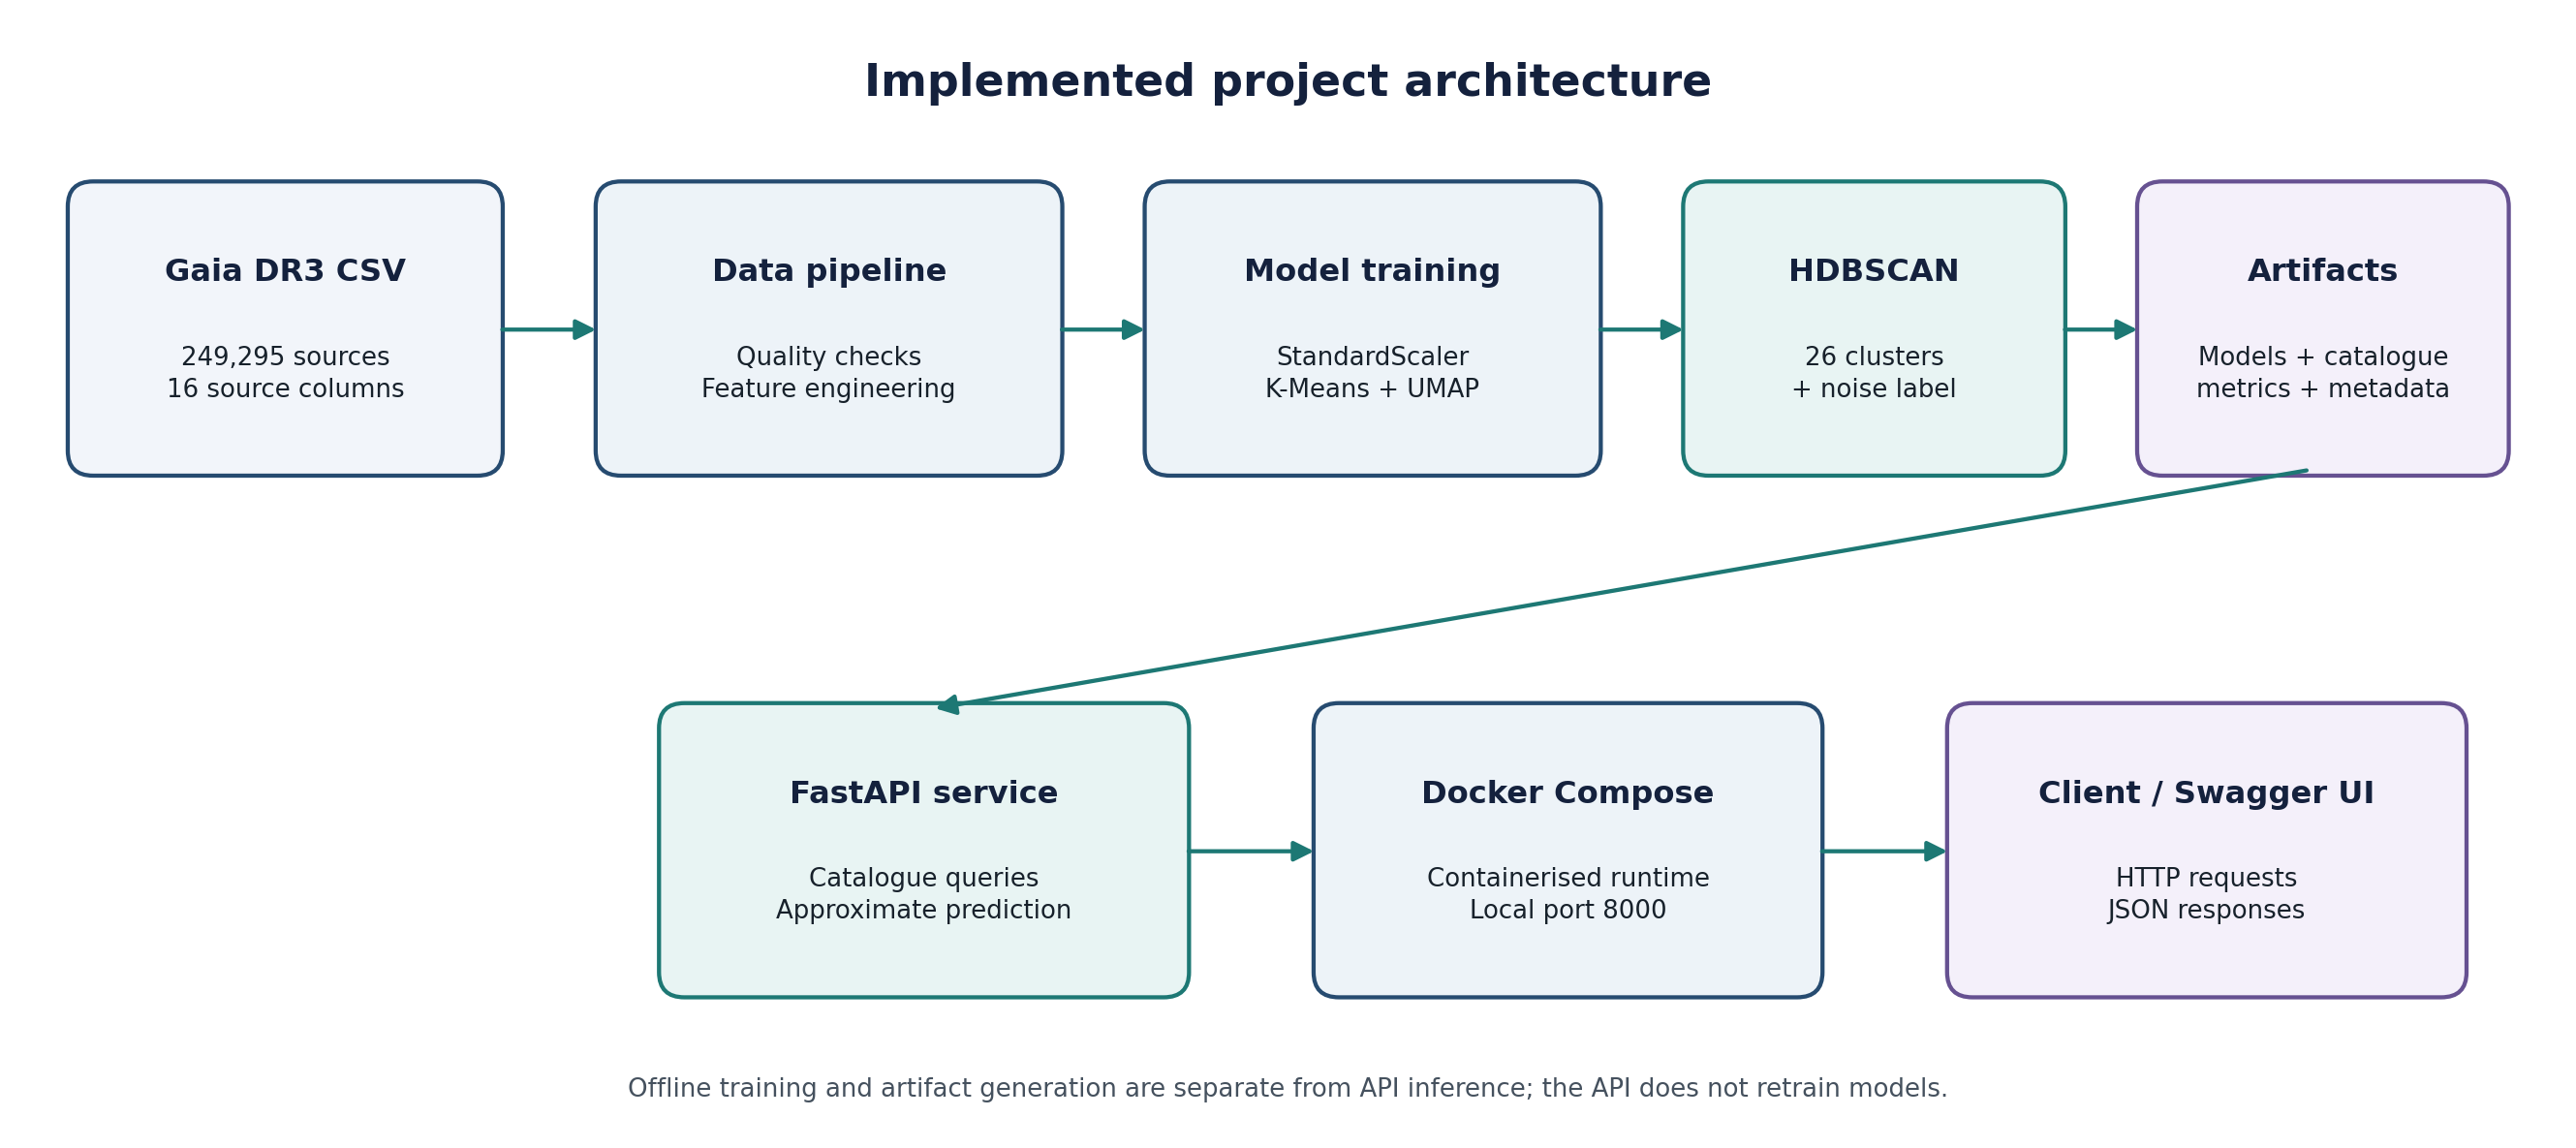
\includegraphics[width=0.96\textwidth,height=4.10cm,keepaspectratio]{image1.png}
\end{center}
\vspace{-1mm}
\begin{block}{Reproducible execution}
 \footnotesize
 Quality rules: RUWE $<1.4$, positive parallax and parallax uncertainty, and parallax SNR $>5$; all 249,295 sources passed in the reported run (zero removed). The six fixed-order features were standardised; fitted estimators were saved and checked; FastAPI and Docker Compose provide the tested local service. \smallcite{\parencite{astropy2013,pedregosa2011}}
\end{block}
\note{\textbf{[About 35 seconds]} The intervention is an engineering pipeline, not just a notebook. The scripted data step checks the schema and four quality conditions: RUWE below 1.4, positive parallax, positive parallax uncertainty, and parallax signal-to-noise above five. All 249,295 records passed those conditions in the reported run, so no rows were removed. The pipeline derives the six features in a fixed order, standardises them, and trains the K-Means and UMAP--HDBSCAN paths. The saved scaler and fitted models are verified separately. FastAPI then loads the saved artifacts for catalogue queries and approximate assignments; Docker Compose runs this service locally. The API does not retrain the models at startup.}
\end{frame}

% =====================================================================
\section{Results}
% =====================================================================

% ---------------------------------------------------------------------
\begin{frame}{The density model groups 15.5\% of sources and leaves 84.5\% unassigned}
\begin{columns}[T]
 \begin{column}{0.54\textwidth}
  \centering
  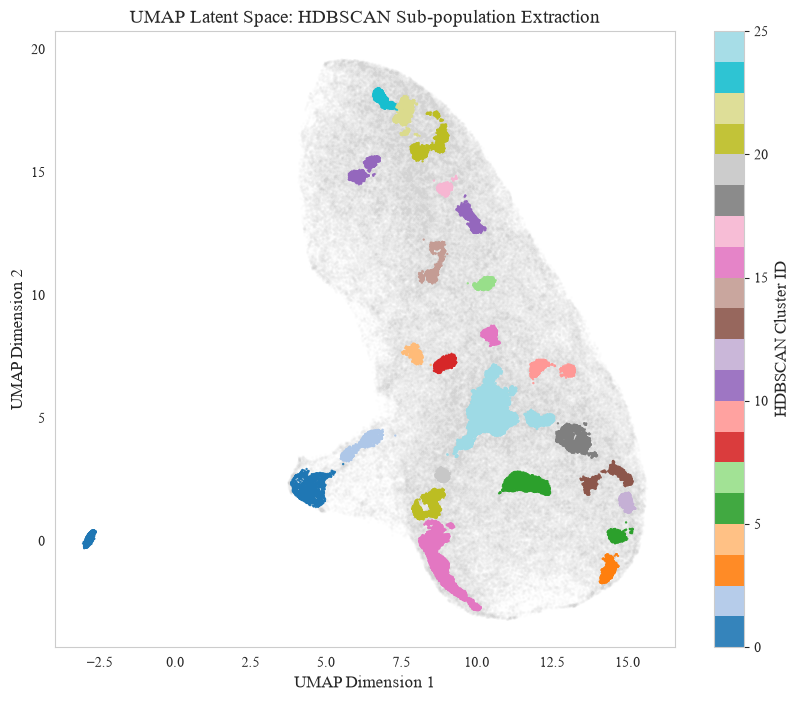
\includegraphics[width=\linewidth,height=5.45cm,keepaspectratio]{image6.png}\\[-1pt]
  {\tiny HDBSCAN labels in the 2D UMAP embedding; grey points are noise/unassigned.}
 \end{column}
 \begin{column}{0.43\textwidth}
  \begin{block}{HDBSCAN outcome}
   \Large\bfseries\color{StrathBlue}26\\[-2pt]
   \normalsize non-noise clusters\\[2pt]
   \large\bfseries 38,640\normalsize\ (15.50\%) assigned\\
   \large\bfseries 210,655\normalsize\ (84.50\%) label $-1$
  \end{block}
  \begin{block}{Internal validation}
   \footnotesize
   \textbf{K-Means silhouette:} $\approx0.3236$ on 10,000 sources in standardised 6D space. \parencite{rouseeuw1987}\\[3pt]
   \textbf{HDBSCAN DBCV:} $0.2178$ on up to 20,000 non-noise sources in 2D UMAP space. \parencite{moulavi2014}
  \end{block}
  {\scriptsize\color{StrathRed}\bfseries The two scores use different algorithms, spaces and samples; do not compare them directly.}
 \end{column}
\end{columns}
\note{\textbf{[About 40 seconds]} The final HDBSCAN setting identifies 26 non-noise groups. Together these contain 38,640 sources, or 15.5 percent of the sample. The remaining 210,655 sources, or 84.5 percent, receive label minus one because they did not meet the selected density criteria in the two-dimensional embedding. This is a major result and a limitation, not something to hide. The K-Means silhouette is about 0.3236, calculated on 10,000 observations in the standardised six-dimensional input space. HDBSCAN's DBCV is 0.2178, calculated on up to 20,000 non-noise observations in the two-dimensional UMAP space. These metrics use different algorithms, spaces and sampling procedures, so their numerical values are not directly comparable. Neither score proves astrophysical identity.}
\end{frame}

% =====================================================================
\section{Conclusion}
% =====================================================================

% ---------------------------------------------------------------------
\begin{frame}{The service works; astrophysical identities remain unverified}
\begin{columns}[T]
 \begin{column}{0.53\textwidth}
  \begin{block}{What was demonstrated}
   \footnotesize
   \begin{itemize}\setlength{\itemsep}{2pt}
    \item Saved scaler, K-Means, UMAP and HDBSCAN artifacts loaded; a 10-row inference smoke test passed.
    \item Docker health check reported 249,295 catalogue rows and all four model components loaded.
    \item Ten local API scenarios and documented Docker-hosted endpoint checks returned HTTP 200.
    \item Prediction assigns to existing fitted groups; it does not discover new clusters.
   \end{itemize}
  \end{block}
  \vspace{1mm}
  {\scriptsize\textbf{Interpretation boundary:} no labelled ground truth or external cross-match was used. Cluster IDs are algorithmic labels, not confirmed stellar populations. The API was tested locally, not cloud-hosted.}
  \par\vspace{4mm}
  {\Large\bfseries\color{StrathNavy}Thank you. Questions?}
 \end{column}
 \begin{column}{0.43\textwidth}
  \begin{block}{Gaia data acknowledgement}
   \fontsize{6.2}{7.5}\selectfont
   This work has made use of data from the European Space Agency (ESA) mission Gaia (\url{https://www.cosmos.esa.int/gaia}), processed by the Gaia Data Processing and Analysis Consortium (DPAC, \url{https://www.cosmos.esa.int/web/gaia/dpac/consortium}). Funding for the DPAC has been provided by national institutions, in particular the institutions participating in the Gaia Multilateral Agreement.
   \vspace{2mm}

   \textbf{Data licence: CC BY-NC 3.0 IGO.}
  \end{block}
  \vspace{1mm}
  {\scriptsize\color{StrathInk!75}Example API assignment: K-Means 3; HDBSCAN 24; membership strength 0.8401 (assignment strength, not a probability).}
 \end{column}
\end{columns}
\note{\textbf{[About 25 seconds]} The software evidence is functional: the saved artifacts load, the Docker health check sees the full catalogue and all four model components, and the tested API requests returned HTTP 200. The prediction endpoint performs approximate assignment to existing fitted clusters; its membership strength is not a calibrated probability. The key scientific boundary is that there is no labelled ground truth or external catalogue cross-match here. Therefore, the clusters are exploratory algorithmic groupings, not confirmed astrophysical identities. The service was tested locally, not deployed as a public cloud API. Thank you; I welcome your questions.}
\end{frame}

\end{document}
